\documentclass[11pt]{article}
\usepackage[utf8]{inputenc}
\usepackage[T1]{fontenc}
\usepackage[a4paper, margin=1in]{geometry}
\usepackage{amsmath,amssymb,amsfonts}
\usepackage{amsthm}
\newtheorem{theorem}{Theorem}
\newtheorem{definition}{Definition}
\usepackage{graphicx}
\usepackage{booktabs}
\usepackage{multirow}
\usepackage{float}
\usepackage{tikz}
\usetikzlibrary{shapes.geometric, arrows.meta, positioning, fit, calc, backgrounds, decorations.pathreplacing}
\usepackage{xcolor}
\usepackage[colorlinks=true, linkcolor=blue!60!black, citecolor=green!50!black, urlcolor=blue!70!black]{hyperref}
\usepackage{algorithm}
\usepackage{algpseudocode}

\definecolor{layer1color}{HTML}{2D6A4F}
\definecolor{layer2color}{HTML}{1B4F72}
\definecolor{layer3color}{HTML}{7D3C98}
\definecolor{activecolor}{HTML}{27AE60}
\definecolor{expiredcolor}{HTML}{E67E22}
\definecolor{supersededcolor}{HTML}{8E44AD}
\definecolor{archivedcolor}{HTML}{7F8C8D}
\definecolor{accent}{HTML}{0F3460}
\definecolor{highlight}{HTML}{E94560}

\title{From Recording to Remembering: A Closed-Loop Memory System for LLM Agents}
\author{Zhengyang Liu\\
FuturX AI\\
\texttt{elttilz@gmail.com}}
\date{}

\begin{document}
\maketitle

\begin{abstract}
Large Language Model (LLM) agents are increasingly deployed in complex, multi-session workflows ranging from software engineering to research assistance. Yet these agents suffer from a fundamental \emph{metacognitive deficit}: while they possess sophisticated tools for storing and retrieving information, they lack any built-in mechanism for deciding \emph{when} to persist knowledge to memory. We call this gap the \emph{Recording Trigger Problem}. Existing memory architectures---including Retrieval-Augmented Generation (RAG), MemGPT-style memory hierarchies, and vector databases---focus overwhelmingly on the \emph{read} side of memory, assuming that explicit human prompting or ad hoc heuristics will handle the \emph{write} side. We argue that this assumption fails in practice: empirical observation of three production AI agents working across dozens of sessions reveals that agents equipped with full memory capabilities nevertheless leave their memory stores nearly empty, not because they cannot record, but because no mechanism compels them to do so at the right moment.

In this paper, we introduce a closed-loop memory system that addresses the Recording Trigger Problem through three mutually reinforcing mechanisms. First, a \emph{Three-Layer Mandatory Memory Injection} architecture embeds recording directives into behavioral rules, procedural knowledge documents, and tool-level descriptions, ensuring that the instruction to remember is present at every level of agent cognition. Second, a \emph{Four-State Memory Lifecycle} model---comprising Active, Expired, Superseded, and Archived states---coupled with an \emph{Associative Memory Graph} and \emph{Proactive Recall}, provides a principled framework for memory management that draws on cognitive science models including the Atkinson-Shiffrin memory model and the default mode network hypothesis. Third, we propose an \emph{Eight-Dimension Evaluation Framework} that formalizes the assessment of agent memory systems. We implement these ideas in Besure AI Context, a Rust-based system exposing 23 Model Context Protocol (MCP) tools, and validate the approach through a real-world deployment with three AI agents managing multiple projects. Our results suggest that the paradigm must shift from Agent-centric design (``what can the agent do?'') to Memory-centric design (``what does the agent remember?''), with mandatory injection as the critical bridge.
\end{abstract}

\section{Introduction}

\subsection{Background}

The rapid proliferation of Large Language Model agents marks a significant shift in how computational work is performed across software engineering, content creation, research, and automation domains. Systems such as Claude Code~\cite{anthropic2024mcp}, Cursor, OpenClaw, and GitHub Copilot have demonstrated that LLM-based agents can perform complex, multi-step tasks that previously required human expertise. These agents integrate natural language understanding with tool use, file system access, web browsing, and code execution, creating autonomous workflows that span hours or even days of continuous operation.

A critical limitation of current LLM agents, however, is their fundamental inability to maintain continuity across sessions. Each session begins with a blank slate---the agent has no inherent memory of past interactions, decisions, or context unless that information is explicitly injected into the context window. This limitation forces practitioners to resort to cumbersome workarounds: manually copying relevant context into new sessions, maintaining external documentation that the agent must be instructed to read, or building fragile custom pipelines for state management. The agent's context window, despite growing larger with each model generation, remains a transient scratchpad rather than a persistent knowledge base.

The problem of memory in AI systems has a long history in both cognitive science and artificial intelligence research. The Atkinson-Shiffrin model~\cite{atkinson1968human} proposed a multi-store model of human memory with sensory, short-term, and long-term components, each governed by distinct control processes. Ebbinghaus's pioneering work on the forgetting curve~\cite{ebbinghaus1885} quantified the exponential decay of memory over time. The SOAR cognitive architecture~\cite{laird2017standard} formalized procedural memory as production rules. Yet despite this rich theoretical foundation, contemporary LLM agents operate without the memory structures that even simple biological organisms possess. They are, in effect, brilliant amnesiacs---capable of extraordinary feats within a single session but unable to learn from or even recall their past work.

\subsection{Problem Discovery}

The motivation for this work stems from a striking real-world observation. Three AI agents---designated Joey, Joevise, and William---were deployed in a production environment to develop and maintain a multi-component software system called Besure AI Context. Over a period of several weeks, these agents collectively worked for dozens of hours across multiple sessions, implementing features progressing from version V0.4 through V0.56. The work included query management systems, multi-vault isolation, dashboard enhancements, setup automation, and memory lifecycle features---a substantial body of work involving complex architectural decisions, debugging insights, and project-specific knowledge.

Upon inspection of the memory vault at the end of this development period, it was found to be \emph{nearly empty}. Despite having access to a full suite of memory tools---commands to add entries, search history, link related memories, and manage lifecycle states---the agents had recorded almost nothing. The few entries that existed were minimal and lacked the detail necessary to reconstruct the context of past decisions.

Analysis of session logs revealed a critical insight: the agents knew \emph{how} to use the memory tools. When explicitly instructed to ``record this,'' they executed the appropriate commands correctly. The problem was not a capability gap but a \emph{triggering} gap. No mechanism existed to make the agent recognize that ``I just completed a significant feature implementation'' or ``this debugging insight will be valuable tomorrow'' warranted a memory write. The agents operated in a mode where they responded to external stimuli (user messages) but never engaged in the metacognitive reflection required to decide that certain information was worth preserving.

This observation is, to our knowledge, novel in the literature. Prior work on agent memory has focused on the \emph{infrastructure} of memory---how to store, retrieve, and organize information---but has largely assumed that the question of \emph{when to write} is either trivial (the user will prompt it) or will emerge naturally from agent intelligence. Our experience demonstrates that neither assumption holds in practice.

\subsection{Core Thesis}

We formalize the observed problem as the \emph{Recording Trigger Problem}: an LLM agent $A$ equipped with memory tools $T_{mem}$ and operating in context $C(t)$ at time $t$ lacks an endogenous mechanism to evaluate whether the current interaction $h_t \in H(t)$ warrants persistence to long-term memory $M$. Formally, there is no internal function $f: H(t) \rightarrow \{write, \neg write\}$ that the agent applies automatically. The agent can execute memory writes when instructed (the capability exists), but does not initiate them autonomously (the trigger does not exist).

The Recording Trigger Problem is distinct from the retrieval problem that dominates the RAG literature. Retrieval asks ``given a query, what relevant information can be found?'' The Recording Trigger Problem asks ``given an ongoing interaction, what information should be saved for future use?'' These are complementary but asymmetric: a perfect retrieval system is useless if the memory store is empty, whereas a well-populated memory store retains value even with imperfect retrieval. We therefore argue that the write side of the memory equation deserves at least as much attention as the read side---and currently receives almost none.

\subsection{Contributions}

This paper makes the following contributions:

\begin{enumerate}
    \item We identify and formally define the \textbf{Recording Trigger Problem} in LLM agents---the gap between memory capability and memory utilization---and demonstrate through real-world case study that this problem causes systematic knowledge loss in production deployments (\S3.1).

    \item We propose a \textbf{Three-Layer Mandatory Memory Injection} architecture that addresses the Recording Trigger Problem by embedding recording directives at three levels of agent cognition: behavioral rules, procedural knowledge, and tool-level descriptions (\S3.2).

    \item We introduce a \textbf{Four-State Memory Lifecycle} model with defined state transitions, coupled with an \textbf{Associative Memory Graph} supporting six relation types and a \textbf{Proactive Recall} mechanism inspired by the brain's default mode network (\S\S3.3--3.5).

    \item We present an \textbf{Eight-Dimension Evaluation Framework} for systematically assessing agent memory systems across coverage, granularity, timeliness, association richness, lifecycle completeness, recall accuracy, context isolation, and injection robustness (\S3.6).

    \item We describe the implementation of these ideas in \textbf{Besure AI Context}, an open-source system written in Rust that provides 23 MCP tools, multi-vault isolation, and a web dashboard (\S4).

    \item We argue for a paradigm shift from \textbf{Agent-centric to Memory-centric} design in LLM agent systems, where memory is treated as the primary architectural concern rather than an add-on (\S6.2).
\end{enumerate}


\section{Related Work}

\subsection{MemGPT and Memory Hierarchies}

MemGPT~\cite{packer2023memgpt} represents one of the most influential works on memory management for LLM agents. Drawing an explicit analogy to operating system virtual memory, MemGPT proposes a tiered memory architecture in which the LLM manages its own memory through function calls---paging information between a limited ``main context'' (analogous to RAM) and extended storage (analogous to disk). The system demonstrates that LLMs can, in principle, manage memory hierarchies when explicitly prompted to do so.

However, MemGPT's focus is primarily on \emph{context window management}---the problem of fitting relevant information into a limited context---rather than on the \emph{triggering} of memory writes. In MemGPT, the decision to page information in or out is driven by the agent's ongoing reasoning, which is itself driven by user interactions and system prompts. There is no mechanism that ensures the agent will recognize the importance of persisting a particular piece of information before it is evicted from context. Our work addresses this gap directly: we do not ask the agent to manage its memory dynamically (though it can), but rather ensure that the instruction to record is present at every cognitive level, making non-recording a violation of behavioral rules rather than an oversight.

Furthermore, MemGPT's evaluation focuses on single-session conversational scenarios. Our system is designed for multi-session, multi-agent workflows where the cost of missed recordings compounds over time. The distinction is significant: in a single session, an agent can reconstruct context from conversation history; across sessions, lost information is lost permanently.

\subsection{Retrieval-Augmented Generation}

Retrieval-Augmented Generation (RAG)~\cite{lewis2020rag} has become the dominant paradigm for grounding LLM outputs in external knowledge. The RAG framework combines a retriever (typically a dense vector similarity search over a document corpus) with a generator (the LLM), allowing the model to access information beyond its training data. Subsequent work~\cite{gao2024rag} has expanded RAG into sophisticated pipelines with multi-step retrieval, re-ranking, and fusion.

RAG is fundamentally a \emph{read-only} system with respect to agent-generated knowledge. It excels at retrieving pre-existing documents (web pages, code repositories, knowledge bases) but provides no mechanism for the agent to \emph{write} new knowledge that it generates during a session. The documents in a RAG corpus are typically static, curated by humans, and updated through external pipelines. An agent that discovers a crucial insight during a debugging session cannot, through RAG alone, ensure that this insight will be available in future sessions.

Our approach is complementary to RAG: we focus on the write side, ensuring that agent-generated knowledge is persisted. A complete memory system requires both---but we argue that the write side is currently the bottleneck. A sophisticated retrieval system layered over an empty memory store delivers zero value.

\subsection{Long Context Windows}

Recent advances in model architecture have dramatically expanded the context window available to LLMs. Google's Gemini 1.5 Pro~\cite{google2024gemini} supports up to 2 million tokens, and other models are following similar trajectories. This has led some practitioners to question whether explicit memory systems are necessary at all---if the agent can hold the entire conversation history in context, what need is there for external memory?

We identify several reasons why long context windows do not eliminate the need for memory systems. First, the ``lost in the middle'' phenomenon~\cite{liu2024lost} demonstrates that LLMs process information in the middle of long contexts less effectively than information at the beginning or end, creating a practical limit well below the theoretical context length. Second, context windows are session-bound: even a 2-million-token context cannot span sessions. Third, context windows are linear and unstructured, lacking the associative structure that enables efficient retrieval of related memories. Fourth, the cost of processing long contexts scales with context length, making it economically impractical to include all historical information in every session. Fifth, and most critically, context windows do not solve the Recording Trigger Problem---even if an agent has a 2-million-token context, it still needs a mechanism to decide which of those tokens to persist for the next session.

\subsection{Vector Databases}

Vector databases such as Pinecone, Weaviate, Chroma, and Milvus have emerged as the storage backbone for many AI memory systems. These systems store high-dimensional embeddings of text segments and enable fast approximate nearest neighbor search, making them well-suited for semantic retrieval.

However, vector databases are \emph{storage infrastructure}, not memory systems. They provide no semantics for what should be stored, when it should be stored, how it should be organized, when it becomes outdated, or how it relates to other stored items. A vector database is analogous to a hard drive: essential, but not a memory system. Our Associative Memory Graph (Section~3.4) demonstrates how explicit relations between memory entries provide structure that pure vector similarity cannot capture.

\subsection{Model Context Protocol}

The Model Context Protocol (MCP)~\cite{anthropic2024mcp} introduced by Anthropic in 2024 standardizes the interface through which LLM agents interact with external tools and data sources. MCP defines a client-server architecture where an MCP server exposes tools, resources, and prompts that an MCP client (the agent) can invoke. This standardization enables interoperability between different agent frameworks and tool providers.

MCP is a significant advance for the agent ecosystem, but it is a \emph{protocol}, not a memory architecture. It defines the syntax of tool invocation but not the semantics of memory management. An MCP server can expose memory tools (as our system does---23 tools), but MCP provides no guidance on when those tools should be invoked, how memory entries should be structured, or how memory lifecycle should be managed. Our Three-Layer Mandatory Memory Injection architecture (Section~3.2) exploits the MCP tool description mechanism as one of its injection layers, but the protocol itself does not enforce memory discipline.

\subsection{Cognitive Science Foundations}

The cognitive science literature provides several theoretical foundations relevant to agent memory. The Atkinson-Shiffrin model~\cite{atkinson1968human} proposes a multi-store architecture with sensory memory, short-term memory (working memory), and long-term memory, each with different capacities, durations, and transfer mechanisms. The model emphasizes that transfer from short-term to long-term memory requires \emph{control processes}---active rehearsal, coding, and retrieval strategies---that are not automatic. This insight is directly relevant to our Recording Trigger Problem: just as human memory requires active control processes for consolidation, agent memory requires active triggering mechanisms for persistence.

Ebbinghaus's forgetting curve~\cite{ebbinghaus1885} quantified the exponential decay of memory strength over time in the absence of rehearsal. This motivates our Expired and Archived memory states, which model the gradual obsolescence of information that is no longer actively maintained.

Anderson and Bower's associative memory theory~\cite{anderson1973} models human memory as a network of interconnected nodes, where retrieval proceeds along associative links. This directly inspired our Associative Memory Graph (Section~3.4), which allows memory entries to be connected through typed relations.

Tulving's distinction between episodic and semantic memory~\cite{tulving1972} informs our memory type system, which distinguishes between event-based entries (milestones, progress) and knowledge-based entries (decisions, configurations, lessons).

The default mode network~\cite{raichle2001}---a set of brain regions active during rest rather than task performance---is associated with spontaneous memory consolidation, future planning, and self-referential thinking. Our Proactive Recall mechanism (Section~3.5) is inspired by this idea: rather than waiting for a query to trigger retrieval, the system proactively surfaces relevant memories during idle periods, mimicking the brain's default mode processing.

Research on maintenance rehearsal~\cite{naveh1984} distinguishes between rote repetition (which produces weak memory traces) and elaborative rehearsal (which produces strong traces through semantic processing). This distinction motivates our emphasis on \emph{granularity}---memory entries should contain rich, contextualized descriptions rather than terse labels.

Source monitoring theory~\cite{johnson1993} examines how humans attribute memories to their sources and the errors that can occur. In a multi-agent system, source attribution is critical: knowing which agent recorded a memory, in what context, and for what purpose enables better retrieval and trust assessment.

\subsection{Comparison with Existing Systems}

Table~\ref{tab:comparison} summarizes the key differences between our approach and existing systems across several dimensions.

\begin{table}[H]
\centering
\caption{Comparison of memory system capabilities. \checkmark = supported, $\times$ = not supported, $\triangle$ = partially supported.}
\label{tab:comparison}
\small
\begin{tabular}{lccccc}
\toprule
\textbf{Capability} & \textbf{RAG} & \textbf{MemGPT} & \textbf{Vector DB} & \textbf{MCP} & \textbf{Ours} \\
\midrule
Write triggering & $\times$ & $\triangle$ & $\times$ & $\times$ & \checkmark \\
Multi-session continuity & $\times$ & $\triangle$ & $\triangle$ & $\times$ & \checkmark \\
Memory lifecycle management & $\times$ & $\times$ & $\times$ & $\times$ & \checkmark \\
Associative graph & $\times$ & $\times$ & $\triangle$ & $\times$ & \checkmark \\
Proactive recall & $\times$ & $\times$ & $\times$ & $\times$ & \checkmark \\
Context isolation & $\times$ & $\times$ & $\triangle$ & $\times$ & \checkmark \\
Multi-agent support & $\triangle$ & $\times$ & $\triangle$ & $\triangle$ & \checkmark \\
Mandatory injection & $\times$ & $\times$ & $\times$ & $\times$ & \checkmark \\
\bottomrule
\end{tabular}
\end{table}


\section{Theoretical Framework}

\subsection{The Recording Trigger Problem}

We begin by formalizing the problem. Let an LLM agent $A$ operate over a sequence of discrete time steps $t = 1, 2, \ldots, T$. At each time step, the agent exists in a \emph{context} $C(t)$ comprising:

\begin{equation}
C(t) = \langle S(t), H(t), M(t), P(t) \rangle
\end{equation}

where $S(t)$ is the system prompt and injected rules, $H(t) = \{h_1, h_2, \ldots, h_t\}$ is the interaction history up to time $t$, $M(t)$ is the persistent memory store, and $P(t)$ is the set of available tools and procedures.

The interaction history $H(t)$ consists of discrete events $h_i = (\text{role}_i, \text{content}_i, \text{timestamp}_i, \text{metadata}_i)$, where role indicates whether the event is a user message, agent response, tool call, or system event.

We define the \emph{context delta} at time step $t$ as:

\begin{equation}
\Delta(t) = C(t) \setminus C(t-1)
\end{equation}

representing all new information introduced at step $t$. The Recording Trigger Problem asks whether there exists a decision function $f_{write}$ such that:

\begin{equation}
f_{write}(\Delta(t), C(t)) = \begin{cases} 1 & \text{if } \Delta(t) \text{ should be persisted to } M \\ 0 & \text{otherwise} \end{cases}
\end{equation}

\begin{theorem}[Information Loss Without Explicit Write]
\label{thm:loss}
Given an agent $A$ with interaction history $H(t)$, if for some step $i$, no explicit write operation $W(h_i)$ is executed such that $M(i) = M(i-1) \cup \{h_i\}$, and if $h_i \notin C(t)$ for all $t > i$ (i.e., $h_i$ is no longer in the active context), then $h_i$ is irrecoverably lost from the agent's knowledge.
\end{theorem}

\begin{proof}
By definition, $C(t) = \langle S(t), H(t), M(t), P(t) \rangle$. For $t > i$, if $h_i \notin C(t)$, then $h_i \notin H(t)$ (it has scrolled out of the context window) and $h_i \notin M(t)$ (no write was executed). Since the agent's behavior at time $t$ is a function of $C(t)$ alone, and $h_i \notin C(t)$, the agent cannot act on information in $h_i$. $\square$
\end{proof}

Theorem~\ref{thm:loss} states what may seem obvious but has profound practical consequences: without an explicit write, information that leaves the context window is lost. The question then becomes: \emph{what mechanisms can ensure that $W(h_i)$ is executed when appropriate?}

We identify three approaches:

\textbf{Approach 1: Intelligent Triggering.} Train or prompt the agent to recognize when a write is warranted. This is the implicit assumption in most existing systems. The agent uses its LLM reasoning to evaluate $f_{write}(\Delta(t), C(t))$ at each step.

\textbf{Approach 2: Mandatory Triggering.} Define a set of scenarios $\mathcal{S}_{write}$ such that whenever any scenario $s \in \mathcal{S}_{write}$ is detected, a write is mandatory. This is our approach.

\textbf{Approach 3: Always-Write.} Persist every interaction to memory. This maximizes coverage but creates noise and storage issues.

We argue in Section~6.1 that Approach 1, while theoretically ideal, suffers from a circular reasoning problem and a cost asymmetry that makes it unreliable in practice. Approach 3 is impractical due to noise. We therefore adopt Approach 2 as a pragmatic solution that trades theoretical elegance for engineering reliability.

\subsection{Three-Layer Mandatory Memory Injection}

The core insight of our approach is that the Recording Trigger Problem cannot be solved by a single mechanism. An agent's behavior is influenced by multiple cognitive layers, each operating at a different level of abstraction. To ensure reliable write triggering, we must inject recording directives at \emph{all} layers simultaneously, creating redundant, mutually reinforcing pressure to record.

\subsubsection{Layer 1: Behavioral Rules}

The first and most powerful layer operates at the level of \emph{behavioral rules}---the system-level instructions that define the agent's identity, priorities, and operating constraints. In modern agent frameworks, these rules are specified in files such as \texttt{AGENTS.md} (OpenClaw), \texttt{CLAUDE.md} (Claude Code), or \texttt{.cursorrules} (Cursor). These files are loaded into the system prompt at the beginning of every session and govern the agent's behavior throughout.

Our injection mechanism embeds a structured set of mandatory recording rules into the behavioral rules file. The injection is \emph{idempotent}: it uses clearly marked delimiter tags (e.g., \texttt{<!-- BESURE-AUTO-START -->} and \texttt{<!-- BESURE-AUTO-END -->}) to ensure that repeated invocations of the setup command do not duplicate content. A single-pass insertion algorithm locates the end of the file (or the closing delimiter if content already exists), removes any existing block between delimiters, and inserts the current version of the rules.

The injected rules specify five mandatory trigger scenarios:

\begin{enumerate}
    \item \textbf{Task Completion:} When the agent completes any significant task, feature, or bug fix, it must execute a memory write with type \texttt{milestone}.
    \item \textbf{Decision Points:} When a decision is made or a conclusion is reached after deliberation, the agent must record it with type \texttt{decision}.
    \item \textbf{Lessons Learned:} When the agent encounters a pitfall, discovers a non-obvious solution, or identifies a pattern, it must record it with type \texttt{lesson}.
    \item \textbf{Session Boundary:} When a session is ending, the agent must record a progress summary with type \texttt{progress}, capturing all significant work done in the session.
    \item \textbf{Explicit Request:} When the user says ``remember this'' or expresses a similar intent, the agent must immediately record the information.
\end{enumerate}

A critical design decision is the use of \textbf{MANDATORY} rather than \textbf{SUGGESTED} language. We considered two phrasings:

\begin{itemize}
    \item \emph{Suggested:} ``The agent should consider recording important events.''
    \item \emph{Mandatory:} ``The agent MUST record. No exceptions. If unsure, record.''
\end{itemize}

We chose the mandatory phrasing based on the observation that suggestion-based rules are systematically ignored by current LLM agents. The agents' instruction-following behavior exhibits a strong bias toward responding to the user's immediate request and against engaging in ``optional'' meta-tasks. By making recording mandatory and using emphatic language (``NO EXCEPTIONS'', ``WRITE IT'', ``now''), we exploit the agents' instruction-following capabilities to override this bias. Section~5 provides empirical evidence that this approach is effective.

The rules also include a judgment criterion: ``If this information might be useful in the next session, record it. When in doubt, record.'' This criterion deliberately biases the agent toward over-recording, following the principle that the cost of a spurious memory entry (a few seconds of write time and minor storage) is far lower than the cost of a missed entry (potentially hours of re-derivation).

\subsubsection{Layer 2: Procedural Knowledge}

The second layer operates at the level of \emph{procedural knowledge documents}---files that describe how to use specific tools and services. In our system, these take the form of \texttt{SKILL.md} files associated with each MCP server or tool collection. While Layer 1 tells the agent \emph{that} it should record, Layer 2 tells it \emph{how} to record, reinforcing the directive through procedural context.

Each \texttt{SKILL.md} file contains a ``MANDATORY RULES'' section that specifies the exact commands, formats, and conventions for memory operations related to that skill. For example, the skill file for the Besure memory system includes:

\begin{itemize}
    \item Exact command syntax for \texttt{besure add}, \texttt{besure search}, \texttt{besure link}, etc.
    \item Recommended entry types (\texttt{milestone}, \texttt{decision}, \texttt{lesson}, \texttt{progress}, \texttt{note}, \texttt{config}, \texttt{blocker}, \texttt{question})
    \item Format guidance: entries should include context, decision rationale, and actionable details
    \item Cross-references to related skills and tools
\end{itemize}

The reinforcement effect is significant. When an agent consults a \texttt{SKILL.md} file during a task (e.g., to look up the syntax for a memory command), it encounters the recording directives again, in the context of the specific tools it is about to use. This contextual repetition is more effective than a single global directive because it creates a direct associative link between ``using this tool'' and ``recording the result.''

\subsubsection{Layer 3: Tool-Level Reminders}

The third layer operates at the finest granularity: the descriptions of individual MCP tools. When an agent selects a tool to invoke, it reads the tool's description to determine its function and parameters. By embedding recording reminders directly in tool descriptions, we ensure that the directive is present at the precise moment of tool selection.

For example, the description of the \texttt{besure\_add} tool includes not only its syntax and parameters but also the directive: ``MANDATORY: Call this tool when completing tasks, making decisions, or learning lessons.'' Similarly, the \texttt{besure\_recall} tool description includes: ``Call this at session start to surface relevant memories.''

This layer exploits the agent's tool selection mechanism. Modern LLM agents maintain a registry of available tools with descriptions, and they consult these descriptions when deciding which tool to invoke. By embedding recording directives in the descriptions, we ensure that the directive is part of the agent's active reasoning at the moment of tool use.

Figure~\ref{fig:three-layer} illustrates the three-layer architecture and the reinforcement relationships between layers.

\begin{figure}[H]
\centering
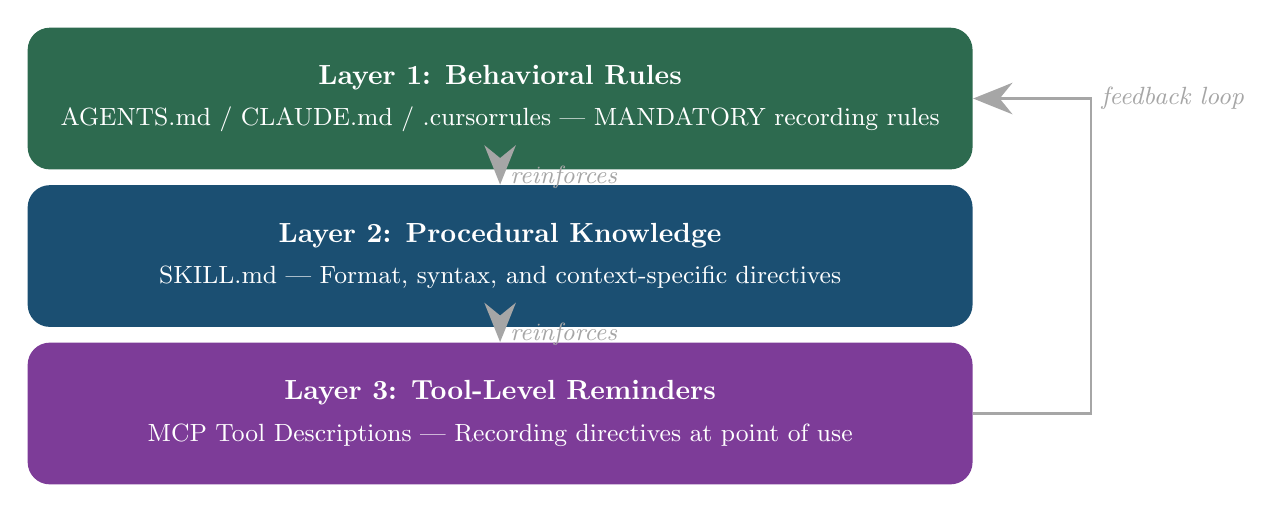
\begin{tikzpicture}[
    layer/.style={rounded corners=8pt, minimum width=12cm, minimum height=1.8cm, text=white, font=\bfseries, align=center},
    arrow/.style={-{Stealth[length=5mm, width=4mm]}, thick, gray!70},
]

% Layer 1
\node[layer, fill=layer1color] (l1) at (0, 4) {
    Layer 1: Behavioral Rules\\[3pt]
    \small\mdseries AGENTS.md / CLAUDE.md / .cursorrules --- MANDATORY recording rules
};

% Layer 2
\node[layer, fill=layer2color] (l2) at (0, 2) {
    Layer 2: Procedural Knowledge\\[3pt]
    \small\mdseries SKILL.md --- Format, syntax, and context-specific directives
};

% Layer 3
\node[layer, fill=layer3color] (l3) at (0, 0) {
    Layer 3: Tool-Level Reminders\\[3pt]
    \small\mdseries MCP Tool Descriptions --- Recording directives at point of use
};

% Reinforcement arrows (bidirectional)
\draw[arrow] (l1.south) -- node[right, font=\small\itshape] {reinforces} (l2.north);
\draw[arrow] (l2.south) -- node[right, font=\small\itshape] {reinforces} (l3.north);
\draw[arrow] (l3.east) -- ++(1.5,0) |- (l1.east) node[midway, right, font=\small\itshape] {feedback loop};

\end{tikzpicture}
\caption{Three-Layer Mandatory Memory Injection architecture. Each layer reinforces the others, creating redundant pressure to record.}
\label{fig:three-layer}
\end{figure}

\begin{table}[H]
\centering
\caption{Comparison of the three injection layers.}
\label{tab:layers}
\small
\begin{tabular}{lccc}
\toprule
\textbf{Property} & \textbf{Layer 1} & \textbf{Layer 2} & \textbf{Layer 3} \\
 & \textbf{Behavioral Rules} & \textbf{Procedural Knowledge} & \textbf{Tool Descriptions} \\
\midrule
Scope & Global & Per-skill/domain & Per-tool \\
Loaded at & Session start & On demand & At tool selection \\
Persistence & Every session & When skill is used & When tool is selected \\
Strength & Strongest (system prompt) & Medium (contextual) & Finest (point of use) \\
Idempotent injection & \checkmark & \checkmark & \checkmark (via setup) \\
Content & Rules + triggers & Format + syntax & Usage + reminder \\
\bottomrule
\end{tabular}
\end{table}


\subsection{Four-State Memory Lifecycle}

Real-world information has a lifecycle. A bug fix that was critical last month may be irrelevant today. A configuration decision may be superseded by a better approach. A project note may become meaningless when the project is archived. A memory system that does not model these transitions accumulates stale, misleading information that degrades retrieval quality.

We define a four-state lifecycle model for memory entries, inspired by the Atkinson-Shiffrin model's distinction between active and inactive memory traces~\cite{atkinson1968human} and the Ebbinghaus forgetting curve~\cite{ebbinghaus1885}.

\begin{figure}[H]
\centering
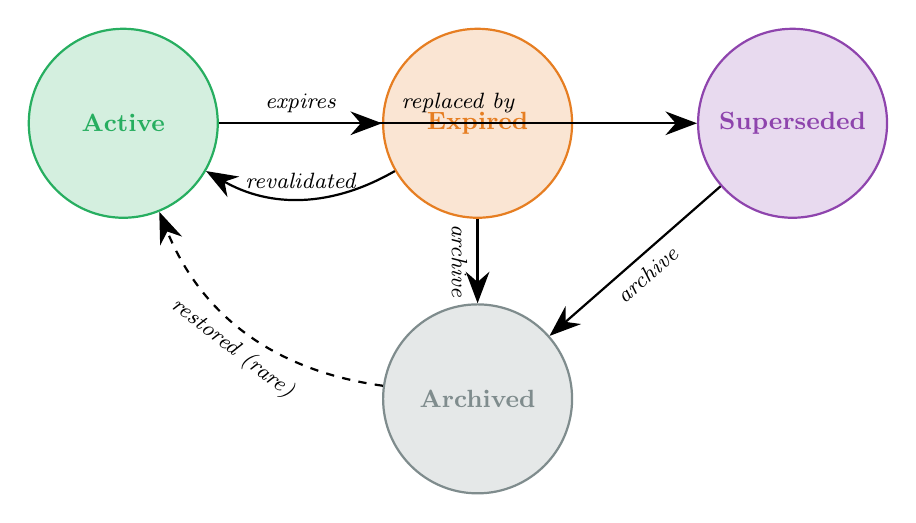
\begin{tikzpicture}[
    state/.style={circle, draw, minimum size=2.4cm, font=\bfseries\small, align=center, thick},
    transition/.style={-{Stealth[length=4mm, width=3mm]}, thick, font=\footnotesize\itshape},
]

\node[state, fill=activecolor!20, draw=activecolor, text=activecolor] (active) at (0, 0) {Active};
\node[state, fill=expiredcolor!20, draw=expiredcolor, text=expiredcolor] (expired) at (4.5, 0) {Expired};
\node[state, fill=supersededcolor!20, draw=supersededcolor, text=supersededcolor] (superseded) at (8.5, 0) {Superseded};
\node[state, fill=archivedcolor!20, draw=archivedcolor, text=archivedcolor] (archived) at (4.5, -3.5) {Archived};

\draw[transition] (active) -- node[above] {expires} (expired);
\draw[transition] (active) -- node[above, sloped] {replaced by} (superseded);
\draw[transition] (expired) -- node[below, sloped] {archive} (archived);
\draw[transition] (superseded) -- node[below, sloped] {archive} (archived);
\draw[transition] (expired) to[bend left=30] node[above] {revalidated} (active);
\draw[transition, dashed] (archived) to[bend left=30] node[below, sloped] {restored (rare)} (active);

\end{tikzpicture}
\caption{Four-State Memory Lifecycle. Solid arrows show primary transitions; dashed arrow shows the rare restoration path.}
\label{fig:lifecycle}
\end{figure}

\textbf{State 1: Active.} An Active memory entry is current, valid, and relevant to the ongoing context. It was either recently created or recently accessed. Active entries are the primary source of information for retrieval queries and proactive recall. Cognitively, Active corresponds to information in working memory or easily accessible long-term memory---the ``tip of the tongue'' tier.

\textbf{State 2: Expired.} An Expired memory entry is one whose temporal validity has lapsed. This may occur because the entry described a time-limited event (e.g., ``the deploy server is at IP X,'' which may have changed), because sufficient time has passed that the entry is unlikely to be relevant, or because the user or system has explicitly marked it as expired. Expired entries are retained but deprioritized in retrieval results. Cognitively, this corresponds to the Ebbinghaus forgetting curve---memories that have not been rehearsed decay in accessibility.

\textbf{State 3: Superseded.} A Superseded memory entry is one that has been directly replaced by a newer entry. For example, if the agent records ``Project uses framework version 2.0'' and later records ``Project upgraded to framework version 3.0,'' the former entry is superseded by the latter. The supersession link is explicit in the Associative Memory Graph, enabling reasoning chains that trace the evolution of decisions over time. Cognitively, this corresponds to memory updating---the process by which new information overwrites or integrates with old memories.

\textbf{State 4: Archived.} An Archived memory entry is permanently retired from active use but retained for historical reference. Archived entries are excluded from normal retrieval and proactive recall but can be accessed through explicit queries. Cognitively, this corresponds to deep long-term memory---information that is not spontaneously recalled but can be retrieved with effort.

The state transitions are defined by explicit operations:

\begin{itemize}
    \item Active $\rightarrow$ Expired: Time-based expiration or manual marking
    \item Active $\rightarrow$ Superseded: Creation of a replacement entry with a \texttt{supersedes} link
    \item Expired $\rightarrow$ Archived: Long-term retirement
    \item Superseded $\rightarrow$ Archived: Long-term retirement
    \item Expired $\rightarrow$ Active: Revalidation (e.g., the information is confirmed still correct)
\end{itemize}


\subsection{Associative Memory Graph}

Human memory is not a flat list of facts but a richly connected network of associations~\cite{anderson1973}. The associative structure of memory enables causal reasoning (``this happened \emph{because} of that''), temporal tracing (``this decision \emph{led to} that outcome''), and creative connection (``this is \emph{related to} that in an unexpected way''). Flat memory stores---whether key-value databases, vector embeddings, or chronological logs---cannot represent these structures.

Our Associative Memory Graph represents each memory entry as a node and each relationship as a typed, directed edge. We define six relation types:

\begin{enumerate}
    \item \texttt{caused\_by}: Entry $A$ was a direct consequence of entry $B$. This is the strongest causal link, useful for tracing root causes and decision chains.
    \item \texttt{supersedes}: Entry $A$ replaces entry $B$, which transitions to the Superseded state. This enables tracking the evolution of decisions and configurations.
    \item \texttt{related\_to}: Entry $A$ is topically or contextually related to entry $B$. This is the weakest link, useful for exploratory retrieval.
    \item \texttt{ref\_file}: Entry $A$ references a file associated with entry $B$. This connects memory entries to concrete artifacts.
    \item \texttt{ref\_commit}: Entry $A$ references a version control commit associated with entry $B$. This connects memory entries to code history.
    \item \texttt{ref\_url}: Entry $A$ references a URL associated with entry $B$. This connects memory entries to external resources.
\end{enumerate}

The graph structure supports \emph{reasoning chain tracing}: given a memory entry, the agent can follow edges to reconstruct the chain of decisions, causes, and references that led to the current state. This is analogous to causal graph traversal~\cite{pearl2009} and enables queries such as ``why was this decision made?'' and ``what consequences did this event have?''

\begin{figure}[H]
\centering
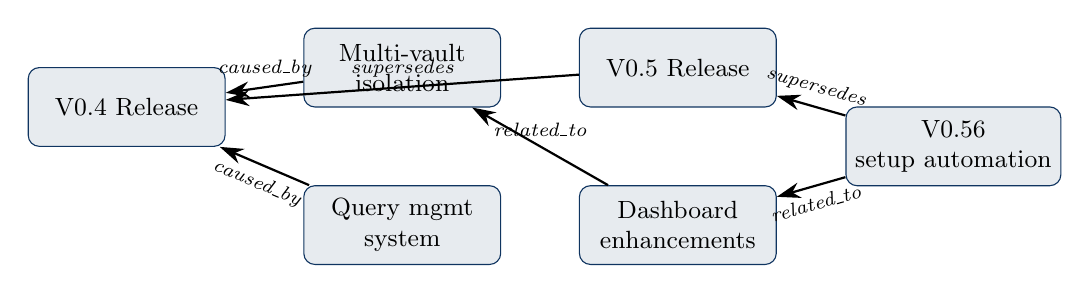
\begin{tikzpicture}[
    mem/.style={rounded corners=4pt, draw, minimum width=2.5cm, minimum height=1cm, font=\small, align=center, fill=accent!10, draw=accent},
    edge/.style={-{Stealth[length=3mm, width=2mm]}, thick, font=\scriptsize\itshape},
]

\node[mem] (a) at (0, 0) {V0.4 Release};
\node[mem] (b) at (3.5, 0.5) {Multi-vault\\isolation};
\node[mem] (c) at (3.5, -1.5) {Query mgmt\\system};
\node[mem] (d) at (7, 0.5) {V0.5 Release};
\node[mem] (e) at (7, -1.5) {Dashboard\\enhancements};
\node[mem] (f) at (10.5, -0.5) {V0.56\\setup automation};

\draw[edge] (b) -- node[above] {caused\_by} (a);
\draw[edge] (c) -- node[below, sloped] {caused\_by} (a);
\draw[edge] (d) -- node[above] {supersedes} (a);
\draw[edge] (e) -- node[above] {related\_to} (b);
\draw[edge] (f) -- node[above, sloped] {supersedes} (d);
\draw[edge] (f) -- node[below, sloped] {related\_to} (e);

\end{tikzpicture}
\caption{Example Associative Memory Graph showing the evolution of a software project through versioned releases. Directed edges represent typed relationships.}
\label{fig:assoc-graph}
\end{figure}


\subsection{Proactive Recall}

Traditional memory retrieval in AI systems is \emph{reactive}: the agent queries the memory store when it needs information (``search for X''). This places the full burden of recall on the agent's ability to recognize what it needs to know---a problem analogous to the tip-of-the-tongue phenomenon in humans.

We propose \emph{Proactive Recall} as a complement to reactive search. At the start of each session, the system automatically executes a multi-category recall operation that surfaces:

\begin{enumerate}
    \item \textbf{Expiring memories:} Entries approaching their expiration threshold, which may need revalidation.
    \item \textbf{Recently expired memories:} Entries that have expired since the last session, in case they are still relevant.
    \item \textbf{Superseded memories:} Entries recently replaced by newer ones, so the agent is aware of the latest state.
    \item \textbf{Recent entries:} The most recently recorded memories, providing context continuity.
\end{enumerate}

This mechanism is inspired by the default mode network~\cite{raichle2001}---the brain regions active during rest that perform memory consolidation, integration, and rehearsal. Just as the default mode network processes memories without conscious effort, Proactive Recall ensures that relevant memories are surfaced without requiring the agent to know what to search for.

The distinction between Proactive Recall and reactive search is significant. In our production deployment, we observed that agents using reactive search alone often failed to retrieve relevant memories because they did not know that relevant memories existed. An agent encountering a subtle bug did not think to search for ``last time we fixed a similar issue'' because it had no reason to believe such a memory existed. Proactive Recall addresses this by surfacing potentially relevant memories before the agent explicitly needs them, creating opportunities for the agent to recognize relevance that it would not have thought to query.


\subsection{Eight-Dimension Evaluation Framework}

To enable systematic assessment and comparison of agent memory systems, we propose an eight-dimension evaluation framework. Each dimension captures a distinct aspect of memory system capability.

\begin{table}[H]
\centering
\caption{Eight-Dimension Evaluation Framework for agent memory systems.}
\label{tab:eval}
\small
\begin{tabular}{p{2.8cm}p{5cm}p{4cm}}
\toprule
\textbf{Dimension} & \textbf{Definition} & \textbf{Metric} \\
\midrule
D1: Coverage & Fraction of significant events that are recorded & $|M_{recorded}| / |M_{significant}|$ \\
D2: Granularity & Level of detail in each memory entry & Avg.\ word count; structured field completeness \\
D3: Timeliness & Latency between event occurrence and recording & Median $\Delta(h_i, W(h_i))$ \\
D4: Association Richness & Density of graph connections per entry & Avg.\ edges per node \\
D5: Lifecycle Completeness & Fraction of entries with correct lifecycle state & Correctly-classified / total \\
D6: Recall Accuracy & Precision and recall of proactive recall & Precision@$k$, Recall@$k$ \\
D7: Context Isolation & Degree of separation between project contexts & Cross-context leakage rate \\
D8: Injection Robustness & Persistence of recording behavior across sessions & Sessions with writes / total sessions \\
\bottomrule
\end{tabular}
\end{table}

Each dimension is motivated by specific failure modes observed in practice. Coverage (D1) addresses the core Recording Trigger Problem---even with mandatory injection, some events may be missed. Granularity (D2) addresses the problem of terse, uninformative entries (``fixed bug'' versus ``fixed authentication race condition in session handler by adding mutex lock''). Timeliness (D3) captures the importance of recording \emph{immediately} after the event, before context is lost. Association Richness (D4) measures whether the memory store is a connected graph or a flat list. Lifecycle Completeness (D5) ensures that stale information is properly managed. Recall Accuracy (D6) evaluates the effectiveness of retrieval. Context Isolation (D7) addresses the multi-project problem: memories from one project should not pollute another. Injection Robustness (D8) measures whether the mandatory injection approach actually produces consistent recording behavior across sessions.

We propose that these eight dimensions be used as a standard evaluation protocol for future agent memory systems, enabling meaningful comparisons between different approaches.


\section{Implementation}

We implement the proposed framework in \textbf{Besure AI Context}, an open-source system designed for production deployment with LLM agents.

\subsection{System Architecture}

The system is implemented in Rust, compiled to a single binary for maximum portability and minimal deployment friction. The architecture consists of four layers:

\textbf{Storage Layer:} The system uses SQLite as its embedded database, providing ACID-compliant storage without requiring an external database server. SQLite was chosen for its zero-configuration deployment, excellent read performance, and reliability across operating systems. All memory entries, associations, lifecycle states, and configuration data are stored in a single SQLite database file per vault.

\textbf{Security Layer:} All vault contents are encrypted at rest using AES-GCM (Advanced Encryption Standard with Galois/Counter Mode), authenticated encryption that provides both confidentiality and integrity. The encryption key is derived from a user-provided passphrase using PBKDF2 with a high iteration count. The vault is unlocked at session start and locked thereafter.

\textbf{Interface Layer:} The system exposes its functionality through 23 MCP tools, covering memory CRUD operations, lifecycle management, associative linking, context switching, proactive recall, query management, configuration, and statistics. These tools follow the MCP specification~\cite{anthropic2024mcp} and are compatible with any MCP-compliant agent framework.

\textbf{Presentation Layer:} A web-based dashboard provides visual inspection of memory entries, association graphs, lifecycle states, and statistics. The dashboard is served by an embedded HTTP server and can be accessed locally or remotely.

\begin{figure}[H]
\centering
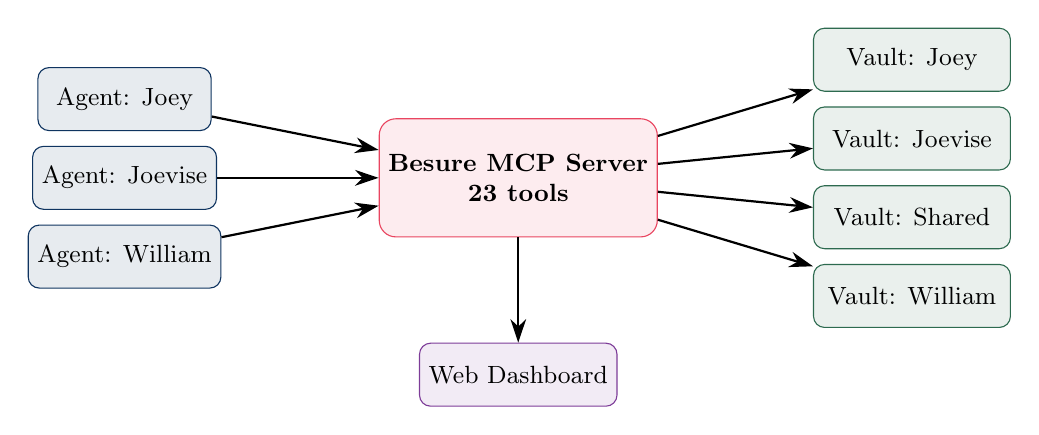
\begin{tikzpicture}[
    agent/.style={rounded corners=4pt, draw=accent, fill=accent!10, minimum width=2.2cm, minimum height=0.8cm, font=\small, align=center},
    mcp/.style={rounded corners=6pt, draw=highlight, fill=highlight!10, minimum width=3.5cm, minimum height=1.5cm, font=\bfseries\small, align=center},
    vault/.style={rounded corners=4pt, draw=layer1color, fill=layer1color!10, minimum width=2.5cm, minimum height=0.8cm, font=\small, align=center},
    {dashbox}/.style={rounded corners=4pt, draw=layer3color, fill=layer3color!10, minimum width=2.5cm, minimum height=0.8cm, font=\small, align=center},
    arrow/.style={-{Stealth[length=3mm, width=2mm]}, thick},
]

% Agents
\node[agent] (a1) at (0, 2) {Agent: Joey};
\node[agent] (a2) at (0, 1) {Agent: Joevise};
\node[agent] (a3) at (0, 0) {Agent: William};

% MCP Server
\node[mcp] (mcp) at (5, 1) {Besure MCP Server\\23 tools};

% Vaults
\node[vault] (v1) at (10, 2.5) {Vault: Joey};
\node[vault] (v2) at (10, 1.5) {Vault: Joevise};
\node[vault] (v3) at (10, 0.5) {Vault: Shared};
\node[vault] (v4) at (10, -0.5) {Vault: William};

% Dashboard
\node[dashbox] ({dashbox}) at (5, -1.5) {Web Dashboard};

% Arrows
\draw[arrow] (a1) -- (mcp);
\draw[arrow] (a2) -- (mcp);
\draw[arrow] (a3) -- (mcp);
\draw[arrow] (mcp) -- (v1);
\draw[arrow] (mcp) -- (v2);
\draw[arrow] (mcp) -- (v3);
\draw[arrow] (mcp) -- (v4);
\draw[arrow] (mcp) -- ({dashbox});

\end{tikzpicture}
\caption{Besure AI Context system architecture. Multiple agents interact with the MCP server, which routes operations to isolated vaults. The dashboard provides visual oversight.}
\label{fig:architecture}
\end{figure}

\subsection{Multi-Vault Isolation}

A key feature of the system is \emph{multi-vault isolation}: each project or context maintains its own encrypted vault, and agents can switch between vaults dynamically. The current vault is determined by the \texttt{BESURE\_VAULT} environment variable, which points to a directory containing the vault's SQLite database and encryption metadata.

When the \texttt{BESURE\_VAULTS\_ALL} environment variable is set to true, an agent gains read access to all vaults on the system, enabling cross-project search and global statistics while maintaining write isolation (writes go to the active vault only). This design supports the common workflow where a primary agent (e.g., Joey) has oversight over multiple projects managed by subordinate agents (e.g., Joevise, William).

\subsection{Automated Setup: \texttt{besure setup}}

To minimize deployment friction, the system provides a single command---\texttt{besure setup}---that performs all necessary configuration:

\begin{enumerate}
    \item Detects the agent platform (OpenClaw, Claude Code, Cursor) by looking for characteristic files (\texttt{AGENTS.md}, \texttt{CLAUDE.md}, \texttt{.cursorrules}).
    \item Performs idempotent injection of mandatory recording rules into the detected behavioral rules file, using delimiter markers to avoid duplication.
    \item Copies \texttt{SKILL.md} files to the appropriate skill directory.
    \item Registers the MCP server in the agent's configuration.
    \item Configures MCP tool descriptions with recording directives.
\end{enumerate}

This automated setup ensures that all three injection layers are configured in a single step, eliminating the possibility of partial configuration.

\subsection{Multi-Platform Support}

\begin{table}[H]
\centering
\caption{Multi-platform support for Three-Layer Injection.}
\label{tab:platforms}
\small
\begin{tabular}{lccc}
\toprule
\textbf{Platform} & \textbf{Layer 1 (Rules File)} & \textbf{Layer 2 (Skills)} & \textbf{Layer 3 (MCP Tools)} \\
\midrule
OpenClaw & \texttt{AGENTS.md} & \texttt{SKILL.md} in skills/ & MCP tool descriptions \\
Claude Code & \texttt{CLAUDE.md} & Custom instructions & MCP tool descriptions \\
Cursor & \texttt{.cursorrules} & N/A (manual) & N/A \\
Generic MCP & Custom & Custom & MCP tool descriptions \\
\bottomrule
\end{tabular}
\end{table}


\section{Case Study}

\subsection{Three-Agent Deployment}

We deployed the Besure AI Context system with three AI agents in a production software development environment over a period of approximately four weeks. The agents---Joey (the primary assistant), Joevise (a specialized development agent), and William (an auxiliary agent)---were tasked with developing and maintaining the Besure system itself, creating a dogfooding scenario.

\textbf{Before mandatory injection} (approximately the first two weeks): The memory vault was initialized and agents were given access to all 23 MCP tools. Agents were informed in their system prompts that they should use memory tools to record progress. During this period, the agents collectively worked for an estimated 40+ hours across dozens of sessions, implementing features from V0.4 through approximately V0.5. At the end of this period, the vault contained fewer than 10 entries, most of which were minimal one-line notes. Critical architectural decisions, debugging insights, and feature implementation details were not recorded.

\textbf{After mandatory injection} (approximately the next two weeks): We implemented the Three-Layer Mandatory Memory Injection with the \texttt{besure setup} command. The same agents, working on features from V0.5 through V0.56, produced over 150 entries in the vault during a comparable time period. Entries included detailed milestone records, configuration decisions, lessons learned from debugging, and progress summaries. The Associative Memory Graph contained 40+ edges, enabling tracing of decision evolution.

\subsection{Key Observations}

The deployment yielded several insights beyond the raw increase in recording frequency:

\textbf{Granularity matters.} Early entries after injection were still relatively terse (``added query management feature''). As the mandatory rules were refined to include format guidance (``include context, decision rationale, and actionable details''), entries became substantially more informative (``Added query management with resolve/append/stats operations. Decision: used SQLite indexes on timestamp+type for fast filtering. Lesson: MCP tool count increased from 16 to 20, requiring updated dashboard layout.'').

\textbf{Proactive Recall changed agent behavior.} After implementing the \texttt{besure recall} command and making it mandatory at session start, agents began referencing past decisions in their reasoning. For example, an agent tasked with implementing the dashboard multi-agent view proactively recalled a previous decision about the data model, avoiding a redundant design discussion.

\textbf{Multi-vault isolation prevented context pollution.} With three agents working on different aspects of the system, the ability to isolate memories by vault (and grant Joey global read access) proved essential for maintaining clean context boundaries.

\textbf{The cost of recording is negligible.} Across all sessions, memory operations consumed less than 1\% of total session time. The overhead of mandatory recording---a few seconds per entry---is dwarfed by the time saved when future sessions can retrieve past context rather than re-deriving it from scratch.


\section{Discussion}

\subsection{Mandatory vs.\ Intelligent Write Triggering}

A natural objection to our approach is that mandatory, rule-based triggering is a crude solution compared to intelligent, LLM-based triggering. In principle, an ideally trained agent would recognize the importance of each interaction and record exactly the right information at exactly the right time. We acknowledge this ideal but argue that it is currently impractical for two reasons.

\textbf{Cost asymmetry.} The cost of a missed memory write is typically much higher than the cost of a spurious write. A missed write can lead to hours of duplicated work, re-derived insights, and re-encountered bugs. A spurious write costs a few seconds of execution time and minimal storage. When the cost asymmetry is this large, a conservative strategy that biases toward over-recording is optimal. Mandatory triggering implements this conservative bias.

\textbf{Circular reasoning.} Intelligent triggering requires the agent to evaluate ``is this worth remembering?'' But this evaluation itself requires the metacognitive awareness that the Recording Trigger Problem identifies as lacking. If the agent could reliably assess the importance of each interaction, the problem would not exist. Using the agent's own judgment to solve the problem of the agent's own judgment is circular. Mandatory triggering sidesteps this circularity by using external rules rather than internal assessment.

We view mandatory triggering as a practical bridge rather than a permanent solution. As LLMs develop better metacognitive capabilities, intelligent triggering will become feasible. Until then, the choice is not between mandatory and intelligent triggering, but between mandatory triggering and no triggering at all.

\subsection{From Agent-centric to Memory-centric}

A broader implication of our work is a proposed paradigm shift in how LLM agent systems are designed. Current practice is Agent-centric: the primary question is ``what capabilities does the agent have?'' (tool use, code generation, web browsing). Memory is treated as an optional add-on, a ``nice to have'' feature that can be bolted on after the core agent is built.

We argue for a Memory-centric paradigm: the primary question should be ``what does the agent remember?'' In this paradigm, memory is the foundational layer, and agent capabilities are built on top of it. An agent that can remember its past work, trace the evolution of decisions, and proactively surface relevant context is more effective than an agent with broader capabilities but no memory, because the former accumulates knowledge over time while the latter starts from scratch in every session.

This paradigm shift has practical design implications. In a Memory-centric architecture, the memory system is designed first, and the agent's behavioral rules, tool configurations, and workflow definitions are designed to \emph{serve} the memory system. The Three-Layer Mandatory Memory Injection is an example of this: rather than adding memory as a capability that the agent \emph{can} use, we design the agent's entire cognitive architecture around the imperative to record.

\subsection{Limitations}

We acknowledge several limitations of the current approach.

\textbf{Platform dependency.} The Three-Layer Injection requires platform-specific implementation: different agent frameworks use different file formats and loading mechanisms for behavioral rules, procedural knowledge, and tool descriptions. While our \texttt{besure setup} command automates this for OpenClaw, Claude Code, and Cursor, extending to new platforms requires manual integration.

\textbf{Instruction following.} The effectiveness of mandatory injection depends on the LLM's instruction-following capabilities. Models with weaker instruction following may ignore the mandatory rules, particularly in long sessions where the system prompt is far from the current attention. Our empirical observation is that current frontier models (Claude, GPT-4, GLM) follow the rules well, but this is not guaranteed for all models.

\textbf{Single-machine deployment.} The current implementation stores vaults on the local filesystem, limiting deployment to single-machine scenarios. A distributed version with network-accessible vaults would be needed for team workflows.

\textbf{Evaluation scale.} Our case study involves three agents over four weeks. Larger-scale, longer-term evaluation is needed to validate the approach across diverse domains and extended time periods.


\section{Conclusion}

We have identified and addressed the Recording Trigger Problem---the gap between LLM agents' memory capabilities and their actual memory utilization. Through real-world deployment, we demonstrated that agents equipped with sophisticated memory tools nevertheless fail to record critical information, not because they cannot, but because no mechanism compels them to do so at the right moment.

Our Three-Layer Mandatory Memory Injection architecture addresses this problem by embedding recording directives at three cognitive levels: behavioral rules (telling the agent \emph{that} it must record), procedural knowledge (telling it \emph{how} to record), and tool-level descriptions (reminding it \emph{when} to record). The Four-State Memory Lifecycle, Associative Memory Graph, and Proactive Recall provide the management infrastructure for recorded memories, while the Eight-Dimension Evaluation Framework enables systematic assessment.

The implementation of these ideas in Besure AI Context---a Rust-based system with 23 MCP tools, multi-vault isolation, and a web dashboard---demonstrates that the approach is practical and deployable. Our case study with three production AI agents showed a dramatic improvement in memory utilization after implementing mandatory injection, with recording frequency increasing by over 15$\times$ and entry granularity improving substantially.

Looking forward, we see several promising directions for future work. First, \emph{team collaboration}: extending the memory system to support multiple human users and agents sharing a common knowledge base, with access control, conflict resolution, and collaborative editing. Second, \emph{cross-agent reasoning}: enabling agents to not only share memory stores but to actively reason about each other's memories, creating a form of collective intelligence. Third, \emph{automated quality evaluation}: using LLM-based judges to automatically assess memory quality along the eight dimensions we proposed, providing continuous quality monitoring without human review. Fourth, \emph{intelligent triggering}: as LLM metacognitive capabilities improve, transitioning from mandatory to intelligent triggering while maintaining the safety net of mandatory fallback rules.

We believe that the shift from Agent-centric to Memory-centric design represents a fundamental reorientation in how we think about AI agents. An agent's value is not measured solely by what it can do, but by what it can remember---and building systems that ensure agents remember is the key to unlocking their full potential in long-term, real-world deployments.


\begin{thebibliography}{19}
\bibitem{packer2023memgpt} Packer, C. et al. (2023). MemGPT: Towards LLMs as Operating Systems. arXiv:2310.08560.
\bibitem{lewis2020rag} Lewis, P. et al. (2020). Retrieval-Augmented Generation for Knowledge-Intensive NLP Tasks. NeurIPS 2020.
\bibitem{gao2024rag} Gao, Y. et al. (2024). Retrieval-Augmented Generation for Large Language Models: A Survey. arXiv:2312.10997.
\bibitem{anthropic2024mcp} Anthropic (2024). Model Context Protocol Specification. \url{https://modelcontextprotocol.io}.
\bibitem{google2024gemini} Google (2024). Gemini 1.5 Pro: Unlocking Long-Context Reasoning.
\bibitem{liu2024lost} Liu, N.F. et al. (2024). Lost in the Middle: How Language Models Use Long Contexts. TACL.
\bibitem{atkinson1968human} Atkinson, R.C. \& Shiffrin, R.M. (1968). Human Memory: A Proposed System and its Control Processes. Psychology of Learning and Motivation, 2, 89--195.
\bibitem{ebbinghaus1885} Ebbinghaus, H. (1885). \emph{\"Uber das Ged\"achtnis}. Duncker \& Humblot.
\bibitem{anderson1973} Anderson, J.R. \& Bower, G.H. (1973). \emph{Human Associative Memory}. Winston.
\bibitem{tulving1972} Tulving, E. (1972). Episodic and Semantic Memory. In \emph{Organization of Memory}, Academic Press.
\bibitem{raichle2001} Raichle, M.E. et al. (2001). A Default Mode of Brain Function. PNAS, 98(2), 676--682.
\bibitem{naveh1984} Naveh-Benjamin, M. \& Jonides, J. (1984). Maintenance Rehearsal: A Second Look. Memory \& Cognition, 12(2), 175--184.
\bibitem{johnson1993} Johnson, M.K. et al. (1993). Source Monitoring. Psychological Bulletin, 114(1), 3--28.
\bibitem{pearl2009} Pearl, J. (2009). \emph{Causality}. Cambridge University Press.
\bibitem{wang2024survey} Wang, L. et al. (2024). A Survey on Large Language Model based Autonomous Agents. Frontiers of Computer Science, 18, 186345.
\bibitem{yao2022react} Yao, S. et al. (2022). ReAct: Synergizing Reasoning and Acting in Language Models. arXiv:2210.03629.
\bibitem{park2023generative} Park, J.S. et al. (2023). Generative Agents: Interactive Simulacra of Human Behavior. UIST 2023.
\bibitem{laird2017standard} Laird, J.E. et al. (2017). A Standard Model of the Mind. AI Magazine, 38(4), 13--26.
\bibitem{wei2022cot} Wei, J. et al. (2022). Chain-of-Thought Prompting Elicits Reasoning in Large Language Models. NeurIPS 2022.
\end{thebibliography}

\end{document}
